\lab{Monte Carlo Integration}{Monte Carlo Integration}
\objective{Implement Monte Carlo integration to estimate integrals. Use Monte Carlo Integration to calculate the integral of the joint normal distribution.}

Some multivariable integrals which are critical in applications are impossible to evaluate symbolically.
For example, the integral of the joint normal distribution
\[
\int_{\Omega} \frac{1}{\sqrt{(2 \pi)^k}} e^{- \frac{\bold{x}^T\bold{x}}{2}}
\]
is ubiquitous in statistics.
However, the integrand does not have a symbolic antiderivative.
This means we must use numerical methods to evaluate this integral. The standard technique for numerically evaluating multivariable integrals is \emph{Monte Carlo Integration}. In the next lab, we will approximate this integral using a modified version of Monte Carlo Integration. In this lab, we address the basics of Monte Carlo Integration.

Monte Carlo integration is radically different from techniques like Simpson's rule. Whereas Simpson's rule is purely computational and deterministic, Monte Carlo integration uses randomly chosen points  in the domain to calculate the integral.
Although it converges slowly, Monte Carlo integration is frequently used to evaluate multivariable integrals because the higher-dimensional analogs of methods like Simpson's rule are extremely inefficient. 

\section*{A Motivating Example}
Suppose we want to numerically compute the area of a circle of radius 1.
From analytic methods, we know the answer is $\pi$.
Empirically, we can estimate the area by randomly choosing points in a $2 \times 2$ square.
The percentage of points that land in the inscribed circle, times the area of the square, should approximately equal the area of the circle (see Figure \ref{fig:MCCircle}).

\begin{figure}
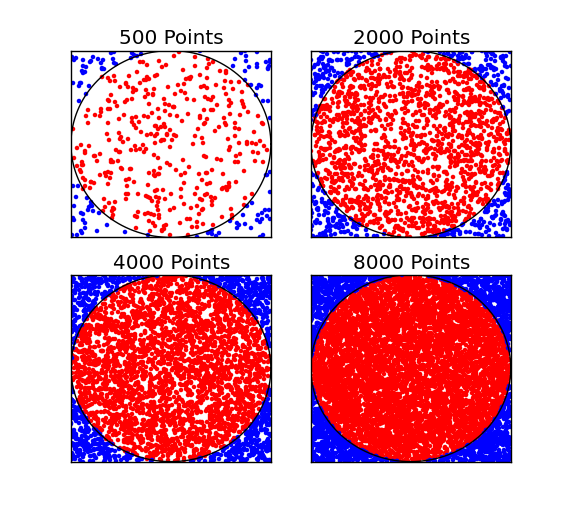
\includegraphics[width=.7\textwidth]{MC.png}
\caption{Finding the area of a circle using random points}
\label{fig:MCCircle}
\end{figure}

We do this in NumPy as follows. First generate 500 random points in the square $[0,1] \times [0,1]$.
\begin{lstlisting}
>>> N = 500 # Number of sample points
>>> points = np.random.rand(2, N)
\end{lstlisting}
We rescale and shift these points to be uniformly distributed in $[-1,1]\times[-1,1]$.
\begin{lstlisting}
>>> points = points*2-1
\end{lstlisting}
Next we determine the number of points in the unit circle.
We compute the Euclidean distance from the origin for each point, then count the points that are within a distance of 1 from the origin.
%The function \li{np.hypot(a, b)} returns the norm of the vector $(a, b)$ where $a$ and $b$ are the $x$- and $y$-components, respectively.
\begin{lstlisting}
>>> # Compute the distance from the origin for each point
>>> pointsDistances = np.linalg.norm(points,axis=0)
>>> # Count how many are less than 1
>>> numInCircle = np.count_nonzero(pointsDistances < 1)
\end{lstlisting}
The fraction of points inside the circle is \li{numInCircle} divided by \li{N}. By multiplying this fraction by the square's area, we can estimate the area of the circle. 
\begin{lstlisting}
>>> circleArea = 4.*(numInCircle/N)
>>> circleArea
3.024
\end{lstlisting}
This differs from $\pi$ by about 0.117.

\begin{problem}
\label{prob:sphere}
Write a function that estimates the volume of the unit sphere. Your function should have a keyword argument \li{N} that defaults to $10^5$. Your function should draw \li{N} points uniformly from $[-1,1]\times[-1,1]\times[-1,1]$ to make your estimate. The true volume is $\frac{4}{3}\pi \approx 4.189$.
\end{problem}

%This demonstrates the main idea of Monte Carlo integration: that random points can be used to estimate a volume. 
%In the next section we will present the generalized method of Monte Carlo integration, which can be used to integrate any function.

\section*{Monte Carlo Integration}

In the examples above, we drew a bounding box around a volume, then used random points drawn from the box to estimate that volume. 
This is easy and intuitive when the volume is a circle or sphere.
But it's hard to generalize this to any arbitrary integral - in order to draw the box, we have to already know something about the volume we are estimating.
Instead, given an arbitrary function $f(x) : \mathbb{R}^n \mapsto \mathbb{R} $ and a region $\Omega \subset \mathbb{R}^n$ in the domain of $f$, we would like to use random points drawn from $\Omega$ to estimate the integral 
$\int_\Omega f(x)\:dV$,
\textit{without} having to specify a bounding box around the volume of integration. 

We can estimate this integral using the approximation.
\begin{equation}\label{equ:mc_eq}
\int_\Omega f(x)\:dV \approx V(\Omega) \frac{1}{N} \sum_{i=1}^N f(x_i)
\end{equation}
where $x_i$ are uniformly distributed random points in $\Omega$ and $V(\Omega)$ is the volume of $\Omega$.
This is the generalized formula for Monte Carlo integration. 

The intuition behind \eqref{equ:mc_eq} is that $\frac{1}{N} \sum_{i=1}^N f(x_i)$ approximates the average value of $f$ on $\Omega$.
We multiply this (approximate) average value by the volume of $\Omega$ to get the (approximate) integral of $f$ on $\Omega$.

For further intuition, compare \eqref{equ:mc_eq} to the Average Value Theorem from single-variable calculus. 
By the Average Value Theorem, the average value of $f(x) : \mathbb{R} \mapsto \mathbb{R} $ on ${[a,b]}$ is given by
\begin{equation}\label{equ:avg_value_eq}
f_{avg} = \frac{1}{b-a}\int_a^b f(x)\:dx.
\end{equation}

If we let $\Omega = {[a,b]}$ in \eqref{equ:avg_value_eq} (noting that $V(\Omega) = b - a$) and replace $f_{avg}$ with the approximation $\frac{1}{N} \sum_{i=1}^N f(x_i)$, then we get precisely the Monte Carlo integration formula in Equation \eqref{equ:mc_eq}!

As it turns out, we can refactor the circle-area problem slightly so that it uses Equation \eqref{equ:mc_eq}. 
Let $f$ be defined by 
$$f(x,y) = \begin{cases} 1 &\mbox{ if $(x$,$y)$ is in the unit circle} \\ 0 &\mbox{ otherwise} \end{cases}$$
and let $\Omega =   {[-1,1]} \times {[-1,1]}$.
The area of the circle is given by 
$\int_\Omega f(x)\:dV$,
which we can estimate with the Monte Carlo integration formula:
\[
\mbox{Area of unit circle } \approx V(\Omega) \frac{1}{N} \sum_{i=1}^N f(x_i) = \frac{4}{N} \sum_{i=1}^N f(x_i).
\]


To summarize, we have the following steps to estimate the integral of any function $f$ over a region $\Omega$ in the domain of $f$:
\begin{enumerate}
\item Draw $N$ random points uniformly distributed in $\Omega$.
\item Find the image of each point under $f$, and take the average of these images.
\item Multiply by the volume of $\Omega$.
\end{enumerate}


\begin{comment}
% Part of the previous explanation of Monte Carlo integration, which was reworked above.
You can calculate the area of the unit circle with the following integration problem:
\[
\mbox{Area of unit circle } = \int_{[-1,1]\times[-1,1]} f(x,y) dA
\]
where
\begin{equation}\label{equ:mc_func}
f(x,y) = \begin{cases} 1 &\mbox{ if $(x$,$y)$ is in the unit circle} \\ 0 &\mbox{ otherwise.} \end{cases}
\end{equation}
%$

This method essentially draws a box around the function to estimate the integral. This works fine if we know the bounds of the function. However, if we don't know the bounds of the function we don't know the dimensions of the box much be to encapsulate the function. 

Luckily, we can still use a random-points method as above to approximate any integral, even if we don't know the bounds. Suppose we wish to evaluate
\[
\int_\Omega f(x)\:dV.
\]
We can approximate this integral using the formula
\begin{equation}\label{equ:mc_eq}
\int_\Omega f(x)\:dV \approx V(\Omega) \frac{1}{N} \sum_{i=1}^N f(x_i),
\end{equation}
where $x_i$ are uniformly distributed random vectors in $\Omega$ and $V(\Omega)$ is the volume of $\Omega$.
This is the formula for Monte Carlo integration. 


In our example, $\Omega$ was the box $[-1,1] \times [-1,1]$ and $f$ was the function defined in \eqref{equ:mc_func}.
Then $\sum_{i=1}^N f(x_i)$ is the number of points in the unit circle, $N$ is the total number of points, and \eqref{equ:mc_eq} is the same as the formula we derived previously.

The intuition behind \eqref{equ:mc_eq} is that $\frac{1}{N} \sum_{i=1}^N f(x_i)$ approximates the average value of $f$ on $\Omega$.
We multiply this (approximate) average value by the volume of $\Omega$ to get the (approximate) integral of $f$ on $\Omega$.

As a 1-dimensional example consider the integral 
\[
\int_0^1 x\,dx \approx (1-0)\frac{1}{N} \sum_{i=1}^N x_i=\frac{1}{N} \sum_{i=1}^N x_i.
\]

The integral on the left-hand-side is $1/2$. 
In the approximation on the right-hand-side, $x_i$ is drawn from a uniform distribution on $[0,1]$. 
The average of $N$ such draws will converge to $1/2$. 

\begin{problem}
\label{prob:crazy_sine}
Monte Carlo Integration is particularly useful when trying to approximate integrals that would be difficult to calculate otherwise. Write a function that approximates the following integral:
$$\int_{1}^{5} \left | \text{sin}(10x)\text{cos}(10x) + \sqrt{x}\text{sin}(3x) \right | dx$$
Your function should accept a keyword argument \li{N} that defaults to $10^5$. Your answer should be approximately $4.502$.
\end{problem}

\end{comment}


\begin{problem}
\label{prob:mc_1d}
Write a function that performs 1-dimensional Monte Carlo integration. 
Given a function $f: \mathbb{R} \mapsto \mathbb{R}$, an interval ${[a,b]}$, and the number of random points to use, your function should return an approximation of the integral
$\int_a^b f(x)\:dx$.
Let the number of sample points default to $10^5$.
Test your function by estimating integrals that you can calculate by hand.

\end{problem}



\begin{problem}
\label{prob:mc}
Generalize Problem \ref{prob:mc_1d} to multiple dimensions. 
Write a function that accepts a function handle $f$ to integrate, the bounds of the interval to integrate over, and the number of points to use. 
Let the number of sample points default to $10^5$.
Your implementation should be robust enough to integrate any function $f$ : $\mathbb{R}^n \mapsto \mathbb{R}$ over any interval in $\mathbb{R}^n$.


Hints:
\begin{enumerate}
\item To draw a random array of points from the given interval, first create a random array of points in $[0,1] \times \ldots \times [0,1]$.
Multiply this array by the dimensions of the interval to rescale it, then add the lower bounds of integration to shift it.
Think about using array broadcasting.

\item You can use \li{np.apply_along_axis()} to apply a function to each column of an array. 
Here is an example of applying a function to points in $\mathbb{R}^2$:

\begin{lstlisting}
>>> points = np.random.rand(2,4)
>>> points
array([[ 0.33144631,  0.52558001,  0.67766158,  0.45570083],
       [ 0.70935864,  0.20985475,  0.25917177,  0.19431292]])
# Apply the norm function to each point
>>> np.apply_along_axis(np.linalg.norm,0,points)
array([ 0.78297275,  0.565927  ,  0.72553099,  0.49539959])
\end{lstlisting}

This is especially useful for functions that don't work nicely with array inputs. 
For example, the code below uses a simple thresholding function \li{f}; calling \li{f(points)} would throw an error, but using \li{np.apply_along_axis} gives the expected result. 
(Note that \li{points} must have at least 2 dimensions for this to work.) 
Refer to the NumPy docs for more information.
\begin{lstlisting}
# Simple function that returns a 0 if x is less than 0.5
>>> f = lambda x: x if x > 0.5 else 0.
# Get 4 random points. The 1 forces the array to be 2-D.
>>> points = np.random.rand(1,4) 
>>> points   
array([[ 0.2144746 ,  0.02490517,  0.86593995,  0.86401139]])
# Evaluate f at each element of points
>>> np.apply_along_axis(f,0,points) 
array([ 0.        ,  0.        ,  0.86593995,  0.86401139])
\end{lstlisting}
%Experiment with this on your own to make sure the function does what you expect. 
%In this example, we chose the axis parameter to be 1 to evaluate the rows of the matrix. 
%If you would like a refresher on axes, see Lab \ref{lab:NumPyArrays}.

\end{enumerate}
\end{problem}

\begin{comment}

\begin{problem}
\label{prob:mc_test}
The exact value of the integral of
\[
f(x,y,z,w) = \text{sin}(x) y^5 -y^3 + zw + yz^3
\]
on $[-1,1]\times[-1,1]\times[-1,1]\times[-1,1]$ is 0.
Run the function \li{mc_int()} you wrote in Problem 3 on $f$ with 100, 1000, and 10000 sample points. Use the default value of 100 iterations for your approximations.
Print the errors of your estimates to the terminal.
\end{problem}

\begin{problem}
The standard normal distribution is an important object of study in probability and statistic.
It is defined by the density function $\frac{1}{\sqrt{2 \pi}} e^{- \frac{x^2}{2}}$.
(Here we are assuming a mean of $0$ and a variance of $1$).
This is a function that cannot be integrated symbolically.
We can use monte carlo integration to estimate the probability that a normally distributed random variable will take a value below a given point.
The probability that the random variable we are considering is less than (or equal to) a given value $x$ is
\[\int_{-\infty}^x \frac{1}{\sqrt{2 \pi}} e^{- \frac{t^2}{2}} dt\]
This function is essentially zero for values of $x$ that lie reasonably far from the mean, so we can estimate this probability by integrating from $-5$ to $x$ instead.

Compare your result at $x = 1$ with the output of the code
\begin{lstlisting}
from scipy.stats import norm
N = norm()
N.cdf(1)
\end{lstlisting}
\end{problem}
\end{comment}



One application of Monte Carlo integration is integrating probability density functions that do not have closed form solutions.

\begin{problem}
The joint normal distribution of $N$ independent random variables with mean 0 and variance 1 is
\[
f(\x) = \frac{1}{\sqrt{2 \pi}^N} e^{- \frac{\x^T\x}{2}}.
\]
The integral of $f(\x)$ over a box is the probability that a draw from the distribution will be in the box.
This is an important distribution in statistics.
However, $f(\x)$ does not have a symbolic antiderivative.
\begin{enumerate}
\item Let $\Omega=[-1.5, 0.75]\times[0,1]\times[0, 0.5]\times[0,1] \subset \mathbb{R}^4$.
Use the function you wrote in Problem \ref{prob:mc} to integrate $f(\x)$ on $\Omega$.
Use 50000 sample points.
\item SciPy has a built in function specifically for integrating the joint normal distribution.
The integral of $f(\x)$ on $B = [-1,1]\times [-1,1]\times[-1,1] \subset \mathbb{R}^3$ can be computed in SciPy with the following code.
\begin{lstlisting}
>>> import scipy.stats as stats

# Define the bounds of the box to integrate over
>>> mins = np.array([-1, -1, -1])
>>> maxs = np.array([1, 1, 1])

# Each variable has mean 0
>>> means = np.zeros(3)

# The covariance matrix of N independent random variables
#    is the NxN identity matrix.
>>> covs = np.eye(3)

# Compute the integral
>>> value, inform = stats.mvn.mvnun(mins, maxs, means, covs)
\end{lstlisting}
Then \li{value} is the integral of $f(\x)$ on $B$.

Use SciPy to integrate $f(\x)$ on $\Omega$. 


\item Return your Monte Carlo estimate, SciPy's answer, and (assuming SciPy is correct) the relative error of your Monte Carlo estimate.
\end{enumerate}
\end{problem}

\section*{Convergence}

The error of the Monte Carlo method is proportional to $1/\sqrt{N}$, where $N$ is the number of points used in the estimation.
This means that to divide the error by 10, we must sample \emph{100 times} more points.

This is a slow convergence rate, but it is independent of the number of dimensions of the problem. 
The error converges at the same rate whether integrating a 2-dimensional or a 20-dimensional function.
This gives Monte Carlo integration an advantage over other methods, and makes it especially useful for estimating integrals in high dimensions.


\begin{figure}
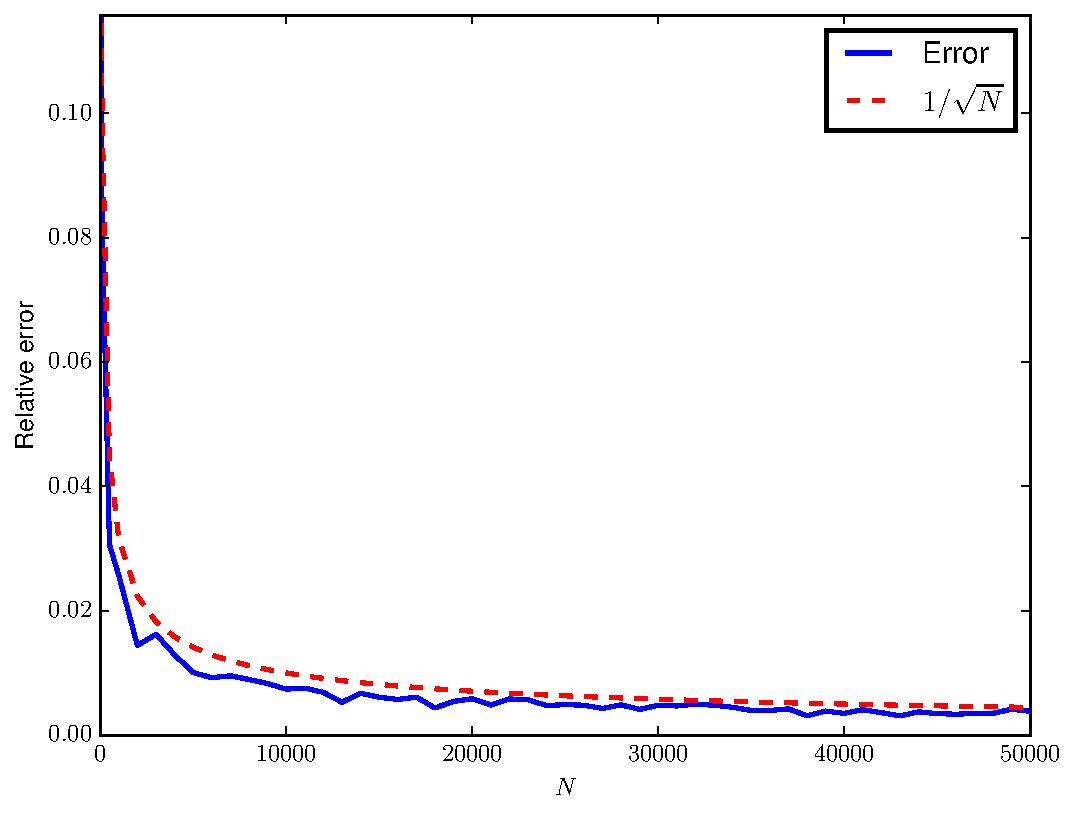
\includegraphics[width=.7\textwidth]{MC_error_2.pdf}
\caption{The Monte Carlo integration method was used to compute the volume of the unit sphere. 
The blue line plots the average error in 50 runs of the Monte Carlo method on $N$ sample points.
The red line is a plot of $1/\sqrt{N}$. }
\label{fig:mc_error_2}
\end{figure}

\begin{problem}
In this problem we will visualize how the error in Monte Carlo integration depends on the number of sample points. 

Run Problem \ref{prob:sphere} with \li{N} equal to 50, 100 and 500, as well as 1000, 2000, 3000, ..., 50000;
having some additional small values of \li{N} will help make the visualization better.

For each value of \li{N}: 
\begin{enumerate}
\item Estimate the volume of the unit sphere using Problem \ref{prob:sphere}, and use the true volume to calculate the relative error of the estimate.
\item Repeat this multiple times to get an average estimate of the relative error. Your function should accept a keyword argument \li{numEstimates} that defaults to 50.
\item Calculate and store the mean of the errors.
\end{enumerate}

Plot the mean relative error as a function of \li{N}. 
For comparison, plot the function $1/\sqrt{N}$ on the same graph.
Your plot should resemble Figure \ref{fig:mc_error_2}).

\end{problem}

\section*{A Caution}
You can run into trouble if you try to use Monte Carlo integration on an integral that does not converge.
For example, we may attempt to evaluate
\[
\int_0^1 \frac{1}{x}\:dx
\]
with Monte Carlo integragtion using the following code.
\begin{lstlisting}
>>> k = 5000
>>> np.mean(1/np.random.rand(k,1))
21.237332864358656
\end{lstlisting}

Since this code returns a finite value, we could assume that this integral has a finite value.
In fact, the integral is infinite.
We could discover this empirically by using larger and larger values of $k$, and noting that Monte Carlo integration fails to converge.

\begin{comment}
\begin{problem}
\label{prob:mc_flawed}
Create a new function (based upon the function from Problem \ref{prob:mc}) that uses a ``flawed'' random number generator that doesn't produce numbers between $-.95$ and $-1$. Test your method on the function from Problem \ref{prob:mc_test}. How bad is the error? 
\end{problem}
\end{comment}
